\chapter{Design}
In this chapter we will explain the applications we developed for this work at a high level. We will skip the experiment automation and plot generation parts of the software, since they are either scripts with a couple of loops that run all the configurations we deemed necessary or simply read data from text files and plot them. Instead, we will be focusing on the two ray tracers we built for this work.

\section{Vulkan Ray Tracer}
\subsection{Rasterized}
The rasterized version of the renderer is quite simple in its design, with a single monolithic Application class handling almost everything and a few helper data structures (Vertex, QueueFamilyIndex, SwapchainSupportDetails and UniformBufferObject) for storing and grouping together information. We see an UML class diagram of this application in figure \ref{rasterized-uml}.

\begin{figure}[hbt!]
  \centering
  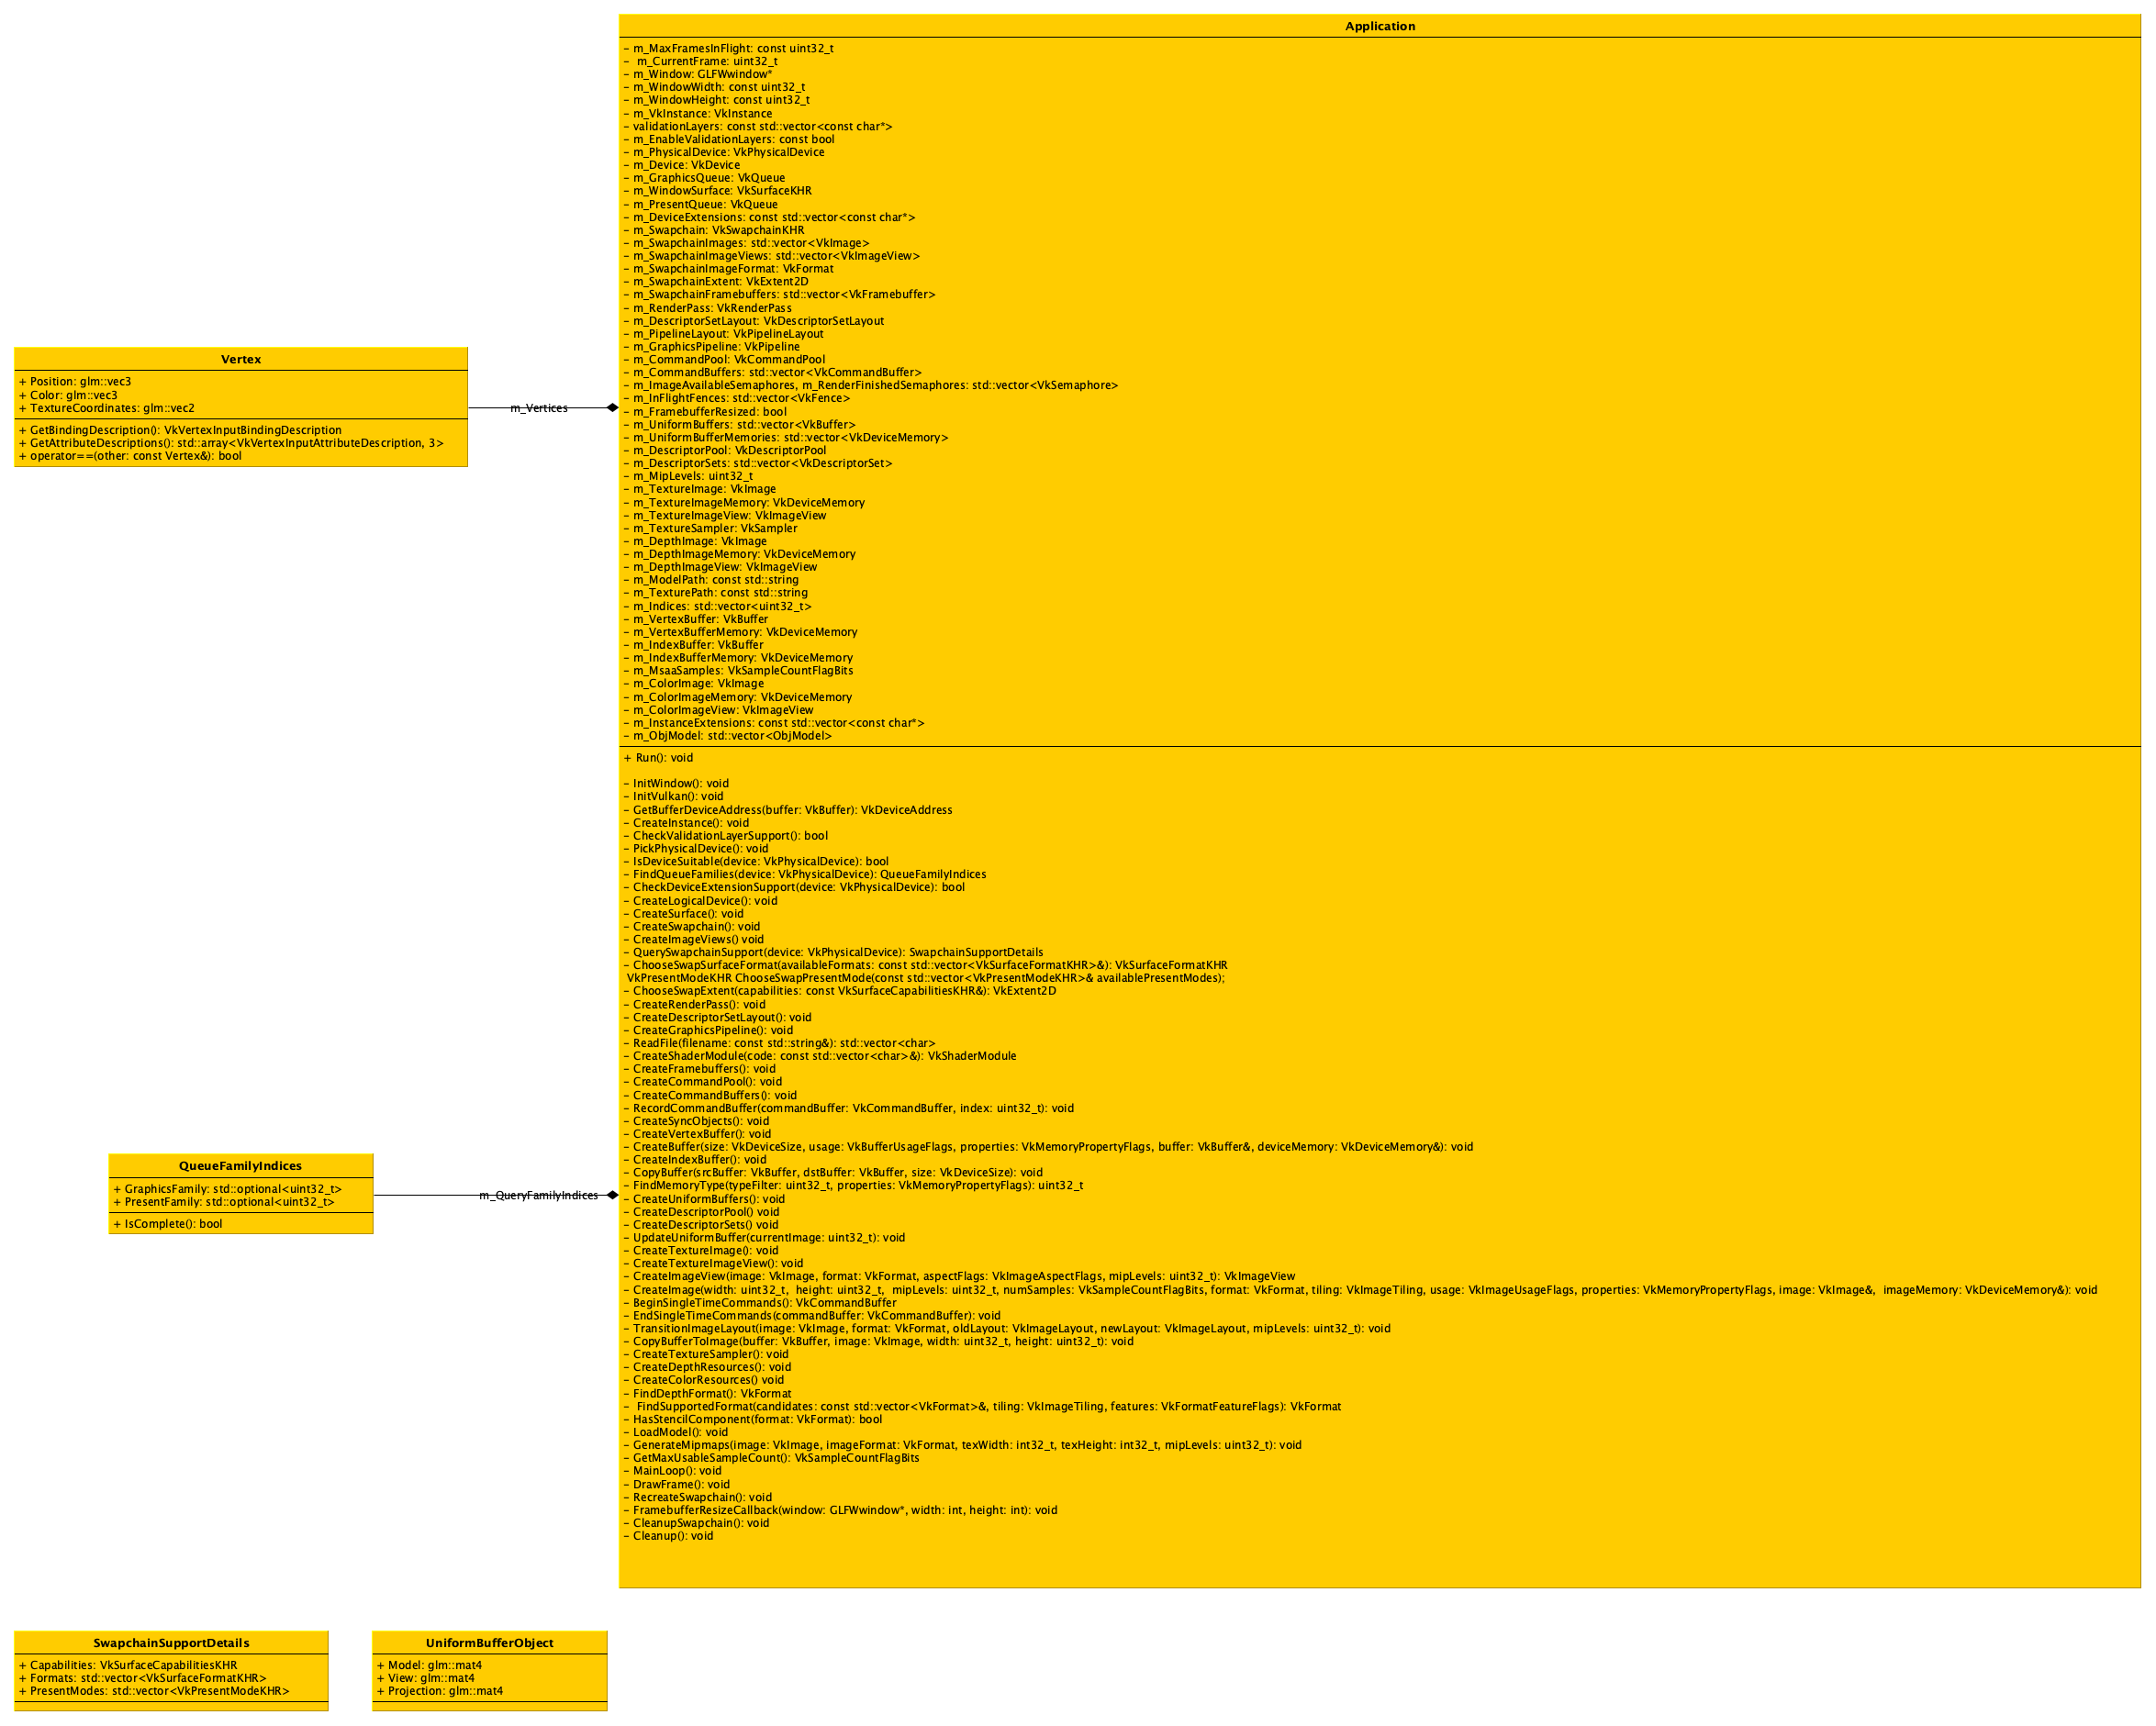
\includegraphics[width=\textwidth]{figuras/rasterized-uml.png}
  \caption{UML class diagram for the rasterized Vulkan renderer.}
  \label{rasterized-uml}
\end{figure}
\subsection{Ray Traced}
\section{OptiX Ray Tracer}
